%%
%% Copyright 2007-2020 Elsevier Ltd
%%
%% This file is part of the 'Elsarticle Bundle'.
%% ---------------------------------------------
%%
%% It may be distributed under the conditions of the LaTeX Project Public
%% License, either version 1.2 of this license or (at your option) any
%% later version.  The latest version of this license is in
%%    http://www.latex-project.org/lppl.txt
%% and version 1.2 or later is part of all distributions of LaTeX
%% version 1999/12/01 or later.
%%
%% The list of all files belonging to the 'Elsarticle Bundle' is
%% given in the file `manifest.txt'.
%%
%% Template article for Elsevier's document class `elsarticle'
%% with harvard style bibliographic references



%% For including figures, graphicx.sty has been loaded in
%% elsarticle.cls. If you prefer to use the old commands
%% please give \usepackage{epsfig}

\makeatletter\if@twocolumn\PassOptionsToPackage{switch}{lineno}\else\fi\makeatother


\usepackage{tabulary,xcolor}
\usepackage{amsfonts,amsmath,amssymb}
\usepackage[T1]{fontenc}
\makeatletter
\let\save@ps@pprintTitle\ps@pprintTitle
\def\ps@pprintTitle{\save@ps@pprintTitle\gdef\@oddfoot{\footnotesize\itshape \null\hfill\today}}
\def\hlinewd#1{%
  \noalign{\ifnum0=`}\fi\hrule \@height #1%
  \futurelet\reserved@a\@xhline}
\def\tbltoprule{\hlinewd{.8pt}\\[-12pt]}
\def\tblbottomrule{\noalign{\vspace*{6pt}}\hline\noalign{\vspace*{2pt}}}
\def\tblmidrule{\noalign{\vspace*{6pt}}\hline\noalign{\vspace*{2pt}}}
\AtBeginDocument{\ifNAT@numbers \biboptions{sort&compress}\fi}
\makeatother

\usepackage{endfloat}

\usepackage{caption}
\captionsetup[figure]{labelsep=none,textformat=empty}
\usepackage{ifluatex}
\ifluatex
\usepackage{fontspec}
\defaultfontfeatures{Ligatures=TeX}
\usepackage[]{unicode-math}
\unimathsetup{math-style=TeX}
\else
\usepackage[utf8]{inputenc}
\fi
\ifluatex\else\usepackage{stmaryrd}\fi


%%%%%%%%%%%%%%%%%%%%%%%%%%%%%%%%%%%%%%%%%%%%%%%%%%%%%%%%%%%%%%%%%%%%%%%%%%
% Following additional macros are required to function some
% functions which are not available in the class used.
%%%%%%%%%%%%%%%%%%%%%%%%%%%%%%%%%%%%%%%%%%%%%%%%%%%%%%%%%%%%%%%%%%%%%%%%%%
\usepackage{url,multirow,morefloats,floatflt,cancel,tfrupee}
\makeatletter


\AtBeginDocument{\@ifpackageloaded{textcomp}{}{\usepackage{textcomp}}}
\makeatother
\usepackage{colortbl}
\usepackage{pifont}
\usepackage[nointegrals]{wasysym}
\urlstyle{rm}
\makeatletter

%%%For Table column width calculation.
\def\mcWidth#1{\csname TY@F#1\endcsname+\tabcolsep}

%%Hacking center and right align for table
\def\cAlignHack{\rightskip\@flushglue\leftskip\@flushglue\parindent\z@\parfillskip\z@skip}
\def\rAlignHack{\rightskip\z@skip\leftskip\@flushglue \parindent\z@\parfillskip\z@skip}

%Etal definition in references
\@ifundefined{etal}{\def\etal{\textit{et~al}}}{}


%\if@twocolumn\usepackage{dblfloatfix}\fi
\usepackage{ifxetex}
\ifxetex\else\if@twocolumn\@ifpackageloaded{stfloats}{}{\usepackage{dblfloatfix}}\fi\fi

\AtBeginDocument{
\expandafter\ifx\csname eqalign\endcsname\relax
\def\eqalign#1{\null\vcenter{\def\\{\cr}\openup\jot\m@th
  \ialign{\strut$\displaystyle{##}$\hfil&$\displaystyle{{}##}$\hfil
      \crcr#1\crcr}}\,}
\fi
}

%For fixing hardfail when unicode letters appear inside table with endfloat
\AtBeginDocument{%
  \@ifpackageloaded{endfloat}%
   {\renewcommand\efloat@iwrite[1]{\immediate\expandafter\protected@write\csname efloat@post#1\endcsname{}}}{\newif\ifefloat@tables}%
}%

\def\BreakURLText#1{\@tfor\brk@tempa:=#1\do{\brk@tempa\hskip0pt}}
\let\lt=<
\let\gt=>
\def\processVert{\ifmmode|\else\textbar\fi}
\let\processvert\processVert

\@ifundefined{subparagraph}{
\def\subparagraph{\@startsection{paragraph}{5}{2\parindent}{0ex plus 0.1ex minus 0.1ex}%
{0ex}{\normalfont\small\itshape}}%
}{}

% These are now gobbled, so won't appear in the PDF.
\newcommand\role[1]{\unskip}
\newcommand\aucollab[1]{\unskip}

\@ifundefined{tsGraphicsScaleX}{\gdef\tsGraphicsScaleX{1}}{}
\@ifundefined{tsGraphicsScaleY}{\gdef\tsGraphicsScaleY{.9}}{}
% To automatically resize figures to fit inside the text area
\def\checkGraphicsWidth{\ifdim\Gin@nat@width>\linewidth
	\tsGraphicsScaleX\linewidth\else\Gin@nat@width\fi}

\def\checkGraphicsHeight{\ifdim\Gin@nat@height>.9\textheight
	\tsGraphicsScaleY\textheight\else\Gin@nat@height\fi}

\def\fixFloatSize#1{}%\@ifundefined{processdelayedfloats}{\setbox0=\hbox{\includegraphics{#1}}\ifnum\wd0<\columnwidth\relax\renewenvironment{figure*}{\begin{figure}}{\end{figure}}\fi}{}}
\let\ts@includegraphics\includegraphics

\def\inlinegraphic[#1]#2{{\edef\@tempa{#1}\edef\baseline@shift{\ifx\@tempa\@empty0\else#1\fi}\edef\tempZ{\the\numexpr(\numexpr(\baseline@shift*\f@size/100))}\protect\raisebox{\tempZ pt}{\ts@includegraphics{#2}}}}

%\renewcommand{\includegraphics}[1]{\ts@includegraphics[width=\checkGraphicsWidth]{#1}}
\AtBeginDocument{\def\includegraphics{\@ifnextchar[{\ts@includegraphics}{\ts@includegraphics[width=\checkGraphicsWidth,height=\checkGraphicsHeight,keepaspectratio]}}}

\DeclareMathAlphabet{\mathpzc}{OT1}{pzc}{m}{it}

\def\URL#1#2{\@ifundefined{href}{#2}{\href{#1}{#2}}}

%%For url break
\def\UrlOrds{\do\*\do\-\do\~\do\'\do\"\do\-}%
\g@addto@macro{\UrlBreaks}{\UrlOrds}



\edef\fntEncoding{\f@encoding}
\def\EUoneEnc{EU1}
\makeatother
\def\floatpagefraction{0.8}
\def\dblfloatpagefraction{0.8}
\def\style#1#2{#2}
\def\xxxguillemotleft{\fontencoding{T1}\selectfont\guillemotleft}
\def\xxxguillemotright{\fontencoding{T1}\selectfont\guillemotright}

\newif\ifmultipleabstract\multipleabstractfalse%
\newenvironment{typesetAbstractGroup}{}{}%

%%%%%%%%%%%%%%%%%%%%%%%%%%%%%%%%%%%%%%%%%%%%%%%%%%%%%%%%%%%%%%%%%%%%%%%%%%
\emergencystretch 20pt \tolerance = 1500 \def\floatpagefraction{0.8}




\makeatletter
\def\ead{\@ifnextchar[{\@uad}{\@ead}}
\gdef\@ead#1{\bgroup
\def\_{\string\underscorechar\space}
\def\{{\string\lbracechar\space}
\def\textdagger{\string\textdagger\space}
\def\texttildeapprox{\string\texttildeapprox\space}
\def~{\hashchar\space}
\def\}{\string\rbracechar\space}
\edef\tmp{\the\@eadauthor}
\immediate\write\@auxout{\string\emailauthor {#1}{\expandafter\strip@prefix\meaning\tmp}}
\egroup
}
%\newcounter{ead}
\gdef\emailauthor#1#2{\stepcounter{ead}
\g@addto@macro\@elseads{\raggedright
\let\corref\@gobble
\eadsep\texttt{#1} (#2)
\def\eadsep{\unskip,\space}}
}

\makeatother

\usepackage{float}

\journal{Nuclear Physics B}


\definecolor{mygreen}{HTML}{E9ECE6}

\newcommand{\figurepath}[1]{figures/#1}

\begin{document}

\begin{frontmatter}
    %% Title, authors and addresses
    %% use the tnoteref command within \title for footnotes;
    %% use the tnotetext command for theassociated footnote;
    %% use the fnref command within \author or \affiliation for footnotes;
    %% use the fntext command for theassociated footnote;
    %% use the corref command within \author for corresponding author footnotes;
    %% use the cortext command for theassociated footnote;
    %% use the ead command for the email address,
    %% and the form \ead[url] for the home page:
    %% \title{Title\tnoteref{label1}}
    %% \tnotetext[label1]{}
    %% \author{Name\corref{cor1}\fnref{label2}}
    %% \ead{email address}
    %% \ead[url]{home page}
    %% \fntext[label2]{}
    %% \cortext[cor1]{}

    \title{A Hierarchical Multilabel Classification Method for Enhanced Thoracic Disease Diagnosis in Chest Radiography}
    \author[label]{Mohammad S. Majdi}
    \author[label]{Jeffrey J. Rodriguez}
    \affiliation[label]{organization={Dept.\ of Electrical and Computer Engineering, University of Arizona},Department and Organization city={Tucson}, postcode={85721}, state={AZ}, country={USA}}

    \begin{abstract}
    Accurate diagnosis of thoracic diseases from chest radiographs is a challenging task that can lead to diagnostic errors with negative patient outcomes. In this study, we propose a novel hierarchical multilabel classification technique that incorporates a conditional loss function to improve the identification of common thoracic diseases in chest radiographic images. The proposed method leverages a predefined disease taxonomy to account for interrelationships among diseases, enhancing the classification performance of machine learning models. Our approach can be seamlessly integrated into existing pre-trained models without the need for re-optimization, ensuring efficiency and broad applicability. To evaluate the effectiveness of the proposed technique, experiments were conducted on several diverse and publicly available datasets, including CheXpert, PadChest, and NIH Chest-Xray14. The results demonstrate that the proposed technique significantly improves the precision and interpretability of machine learning models for thoracic disease on chest radiography. This approach has the potential to promote an accurate and efficient diagnosis by providing radiologists with an additional layer of decision support, ultimately leading to better patient outcomes.
    \end{abstract}

    \begin{keyword}  Chest radiography, hierarchical classification, disease taxonomy, multi-label classification, conditional loss function, diagnostic errors, machine learning, medical imaging \end{keyword}

\end{frontmatter}


\section{Introduction}

Hierarchical multi-label classification methods have been successfully implemented in a variety of domains, including text processing~\cite{aly_Hierarchical_2019}, visual recognition~\cite{bi_Mandatory_2014}, and genomic analysis~\cite{bi_BayesOptimal_2015}. A common technique~\cite{chen_Deep_2019} for exploiting such a hierarchy is to train a classifier on conditional data while ignoring all samples with negative parent-level labels and then reintroducing these samples to fine-tune the network across the entire dataset~\cite{chen_Deep_2019}. These approaches help the classifier focus on the relevant data during initial training, improving prediction accuracy. It also allows the classifier to consider label hierarchies. However, these techniques are computationally expensive, as they require training a classifier on conditional data and then fine-tuning it on a full dataset. This makes them difficult to apply to real-world problems, where the amount of data is often very large. Additionally, they may not always perform satisfactorily, as it may not be possible to find a good set of parent-level labels that accurately capture the hierarchical relationships in the data. Another common strategy is cascading architecture where different classifiers are trained at each level of the hierarchy. Although these techniques enable more granular data analysis (each classifier can focus on a specific level of the hierarchy), they require a substantial amount of computational resources. Other existing deep learning-based approaches often use complex combinations of CNNs and recurrent neural networks (RNNs)~\cite{guo_CNNRNN_2018,kowsari_HDLTex_2017}.

We propose a method that takes advantage of hierarchical relationships between labels without imposing computational requirements. Our proposed method is adaptable to the computational capacity of the user. If sufficient computational resources are available, it can be used as a standalone loss function during the optimization process, or it can be applied to test samples without the need to fine-tune the pre-trained ML model. The proposed loss function is based on the following hypothesis.

\begin{itemize}
    \item  The highest level of taxonomy contained the most general labels, whereas the lowest level contained the least.
    \item  Each node contains a collection of granular child labels.
\end{itemize}


\section{Methods}
In this section, we present a comprehensive methodology to enhance multi-label classification performance using chest radiograph (CXR) data, which is applicable not only during the training phase, but also as a transfer learning approach during the testing phase. Our proposed strategy encompasses the formulation of a multi-label classification problem for CXR, the establishment of an evaluation protocol, and the incorporation of a loss measurement technique that leverages hierarchical label relationships. As a transfer learning approach, our method facilitates the adaptation and fine-tuning of pre-trained models, thereby augmenting their generalizability to novel tasks. This ultimately contributes to the improvement of disease diagnosis and treatment through increased accuracy in detecting abnormalities within CXR images.



\subsection{Notations}
Let us denote the following parameters:

\begin{itemize}

    \item  $\mathcal{C} = {\{c_k\}}_{k=1}^{K} , c_k \in \{0,1\} $: the set of classes (categories) in the multi-label dataset, where $c_k $ is the name of the $k $-th class.

    \item  $\mathcal{E} $: set of directed edges representing parent-child relationships between classes.

    \item  $y_k^{(i)} \in \{0,1\} $: true label for the $k $-th class$(c_k) $ of instance $i $.

    \item  $q_k^{(i)} \in \left( -\infty,0 \right) $: logits obtained in the last layer of the neural network model before the sigmoid layer.

    \item  $p_k^{(i)} = \text{sigmoid}\left(q_k^{(i)}\right) = \frac{1}{1+\exp{\left(-q_k^{(i)}\right)}} $: predicted probability for the $k $-th class ($c_k) $ of instance $i $ with a value between 0 and 1. $p_k^{(i)} $ represents the likelihood that class $k $ is present in instance $i $ and is obtained by passing logits $q_k^{(i)} $ through a sigmoid function.

    \item  $\theta_k $: Binarization threshold for class $k $. To obtain this, we can utilize

    \item  $t_k^{(i)}=\left\{\begin{array}{lc}1&\text{if}\;p_k^{(i)} \geq \theta_k\\0&\text{otherwise.}\end{array}\right. $: predicted label obtained by binarizing the $p_k^{(i)} $

    \item  ${\widehat p}_k^{(i)} \in (0,1) $: updated predicted probability for the $k $-th class of instance $i $ with a value between 0 and 1.

    \item  $t_k^{(i)}=\left\{\begin{array}{lc}1&\text{if}\;p_k^{(i)}\geq\theta_k\\0&\text{otherwise.}\end{array}\right. $: updated predicted label for the $k $-th class of instance $i $.

    \item  $\ensuremath{K} $: number of categories (aka classes) in a multi-class, multi-label problem. For example, if we have a dataset that is labeled for the presence of cats, dogs, and rabbits in any given image. If a given image $X^{(i)} $ has cats and dogs but not rabbits, then $Y^{(i)} = \{1,1,0\} $.

    \item  $N $: Number of instances.

    \item $X^{(i)} $: Data for the $i $-th instance.

    \item $Y^{(i)} = {\left\{ y_k^{(i)}\right\}}_{k=1}^{K} $: true label set, for instance $i $.

    \item  $P^{(i)} = {\left\{p_k^{(i)}\right\}}_{k=1}^{K} $: predicted probability set, for instance $i $.

    \item  $T^{(i)} = {\left\{t_k^{(i)}\right\}}_{k=1}^{K} $: predicted label set, for instance $i $.

    \item  $\mathbb{X} = {\left\{X^{(i)}\right\}}_{i=1}^{N} $: Set of all instances.

    \item  $\mathbb{Y} = {\left\{Y^{(i)}\right\}}_{i=1}^{N} $: Set of all true labels.

    \item  $\mathbb{D} = \left\{\mathbb{X},\mathbb{Y} \right\} $: Dataset containing true labels.

    % \item  $\mathbb{D}_{\text{phase1}},\mathbb{D}_{\text{phase2}} $: randomly selected subsets of the $\mathbb{D} $ dataset used for phase1: training the machine learning model and phase2: applying the proposed taxonomy technique. $\mathbb{D}_{\text{phase1}}\cup\;\mathbb{D}_{\text{phase2}}=\mathbb{D} $ and $\mathbb{D}_{\text{phase1}} \bigcap \mathbb{D}_{\text{phase2}} = \varnothing $

    % \item  $\mathbb{D}_{\text{phase1}}^{\text{train}} $ , $\mathbb{D}_{\text{phase1}}^{\text{test}} $: Train and test datasets randomly selected from $\mathbb{D}_{\text{phase1}} $ where $\mathbb{D}_{\text{phase1}}^{\text{train}}\bigcup \mathbb{D}_{\text{phase1}}^{\text{test}}=\mathbb{D}_{\text{phase1}} $ and $\mathbb{D}_{\text{phase1}}^{\text{train}}\bigcap
    % \mathbb{D}_{\text{phase1}}^{\text{test}}=\varnothing $

    % \item  $\mathbb{D}_{\text{phase2}}^{\text{train}} $ , $\mathbb{D}_{\text{phase2}}^{\text{test}} $: Train and test datasets randomly selected from $\mathbb{D}_{\text{phase2}} $ where $\mathbb{D}_{\text{phase2}}^{\text{train}}\bigcup \mathbb{D}_{\text{phase2}}^{\text{test}}=\mathbb{D}_{\text{phase2}} $ and $\mathbb{D}_{\text{phase2}}^{\text{train}} \bigcap \mathbb{D}_{\text{phase2}}^{\text{test}} = \varnothing $

    \item  $\mathcal{L} \left(y_k^{(i)},p_k^{(i)}\right) $: $\mathcal{L} $ is an arbitrary loss function (e.g., binary cross entropy) that takes the true label and predicted probability for class k and instance I~and outputs the loss value $l_k^{(i)} $. We will refer to this as the ``base loss function'' throughout this paper.

    \item  $\text{Loss}(\theta) $: Measured loss in all cases and instances. This value will be obtained using a modified version of the base loss function $\mathcal{L}(\cdot) $ (e.g., with added regularization, etc.).

    \item  $\mathcal{G}=\left\{\mathcal{C},\mathcal{E}\right\} $: directed acyclic graph (DAG) $\mathcal{G} $ represents the taxonomy of thoracic diseases, where $\mathcal{C} $ is the set of disease classes and $E $ is the set of directed edges representing parent-child relationships between these classes.

    \item  $\Lambda(c_k)\subset \mathcal{C}$: set of parent classes of class $c_k $ in DAG $\mathcal{G} $.

    \item  $\mathcal{J}(c_k) \subset \mathcal{C}$: set of child classes of class $c_k $ in DAG $\mathcal{G} $

    \item  $\omega_k^{(i)} $: Estimated weight for $k$-th class $c_k $ of instance $i $ with respect to its parent class $\Gamma_k $.

    \item  ${\widehat l}_k^{(i)} = \omega_k^{(i)} \; l_k^{(i)} $: updated loss for class $k $ and instance $i $.

    \item  ${\widehat p}_k^{(i)}=\omega_k^{(i)}\;p_k^{(i)} $: updated predicted probability for the $k $ -th class.

\end{itemize}


\subsection{Problem Formulation}

Let us define the multi-label classification problem as follows. Let $\mathbb{X} = {\left\{X^{(i)}\right\}}_{i=1}^{N} $ be the set of $N $ chest radiograph images and $\mathbb{Y} = {\left\{Y^{(i)}\right\}}_{i=1}^{N} $ be their corresponding ground truth labels. In the context of chest radiograph interpretation, the label set $\mathcal{C} $ typically includes various thoracic abnormalities such as pneumothorax, consolidation, atelectasis, and cardiomegaly. The ground-truth labels for the dataset were provided by experienced radiologists who annotated each image with the corresponding abnormalities.

Given the set of disease classes $\mathcal{C} = \{c_1,c_2,\dots,c_K\} $, let us define a directed acyclic graph (DAG) $\mathcal{G}=\left\{\mathcal{C},\mathcal{E}\right\} $ representing the taxonomy of thoracic diseases, where $E $ is the set of directed edges representing parent-child relationships between these classes. For each node $c_k \in \mathcal{C} $, let $\Lambda (c_k) \in \mathcal{C} : c_k \neq \Lambda(c_k) $ the parent node of class $c_k $ and denote $\mathcal{J} (c_k)\subset \mathcal{C} $ the set of child classes of class $c_k $ in DAG $\mathcal{G} $. The root node does not represent an abnormality (ie, normal chest radiograph).

Let $\omega_k^{(i)} $ be a scalar weight assigned to the class $c_k $ of instance $i $ with respect to its parent class $\Lambda(c_k) $. In multi-label classification problems, each sample can have multiple labels simultaneously assigned to it; thus, the sigmoid function is utilized to predict the probabilities for each class being present in a given sample. The output of the final layer of the neural network, for instance $i $, is passed through a sigmoid function to generate a set of values between 0 and 1 corresponding to the label set $\mathcal{C} $ to obtain a set of $K $ predicted probabilities $P^{(i)}={\left\{p_k^{(i)}\right\}}_{k=1}^{K} $. These predicted probabilities, derived from the sigmoid activation function, can be interpreted as the probability that the input sample belongs to each class. Consequently, the loss function quantifies the similarity between predicted and true labels.

Let us denote $l_k = \mathcal{L} \left(p_k^{(i)},y_k^{(i)}\right),\hspace{0.33em}k \in \{1,2,\dots,K\} $ where $\mathcal{L}(\cdot) $ is an arbitrary and appropriate single class loss function for the task (e.g., binary cross-entropy, Dice, etc.) that is used to calculate the difference between the predicted probability $p_k^{(i)} $ and the true class label $y_k^{(i)} $ for sample $X^{(i)} $ and class $k $.



\subsection{Label Taxonomy and Hierarchy}
To exploit the inherent hierarchical relationships between thoracic abnormalities, the first step is to define a disease taxonomy that demonstrates different abnormalities~interrelationships. In this taxonomy, diseases will be structured hierarchically, with higher levels representing broader disease categories and lower levels representing more nuanced distinctions between related diseases. For example, pleural effusion and pneumothorax can be categorized as subcategories of pleural abnormalities, whereas atelectasis and consolidation can be classified under pulmonary opacity. This hierarchical structure enables the model to take advantage of the relationships between diseases to improve its classification performance.

In medical imaging, labels are frequently organized as trees or directed acyclic graphs (DAGs) to represent the hierarchical relationships between different classes of labels. For example, a DAG can be used to represent the human body's organs, with each node representing a different organ, and the edges representing the relationships between organs (e.g., the liver is part of the abdominal cavity). Using a tree or DAG structure for labels in medical imaging has a number of advantages, including improved accuracy and interpretability of classification algorithms, which are essential for making sense of the vast amounts of data generated by medical imaging technologies. In medical imaging, hierarchies of labels are typically constructed by subject matter experts with a comprehensive understanding of human anatomy and physiology, such as radiologists. Construction of these hierarchies can be challenging and time-consuming because it requires in-depth knowledge of the subject matter and the ability to organize complex data into clean and intuitive structures.

To develop a comprehensive label taxonomy for lung diseases, we integrated the taxonomies presented by Irvin~\cite{irvin_CheXpert_2019} for the CheXpert dataset and Chen~\cite{chen_Deep_2020} for the PadChest and PLCO datasets. This unified taxonomical structure can be applied to various chest radiography datasets. In the following two sections, we propose two methods for incorporating taxonomy information to improve accuracy.

\begin{itemize}
    \item In the first approach, we use taxonomy information to update the predicted probability of each class based on the predicted probability of its respective parent classes. This method can be easily applied unsupervised to existing, pre-trained models without the need for true labels.

    \item  In our second approach, we propose a similar concept. However, rather than directly updating the predicted probability of each class, we instead update the loss value of each class based on the loss values of its parent classes.
\end{itemize}

\subsection{Approach 1: Conditional Predicted Probability}A transfer learning-based approach that uses hyperparameters to update the predicted probability of a class based on the predicted probability of its parent class can be devised to further enhance the accuracy of classification by considering the interrelationship between different classes. In this approach, our aim is to calculate the conditional predicted probability for each class $k $ and instance $i $, taking into account the predicted probabilities of the parent class. We can formalize this by defining a new predicted probability for the $k $ -th class $(c_k) $ and instance $i $ as follows.

\begin{equation}
    \widehat{p}_k^{(i)} = \frac{1}{ 1 + \exp \left(-\left(q_k^{(i)} + \alpha_{k,j} q_j^{(i)} \right)\right) }
    \label{Taxonomy.Eq.Taxonomy.Eq.1.pred.approach1}
\end{equation}

where $j $ is defined so that $c_j=\Lambda(c_k) $, and $\alpha_{k,j} $ is the hyperparameter controlling the influence of different parent class logits on child class logits. When $\alpha_{k,j}=0 $, there is no influence from the parent classes, and when $\alpha_{k,j}>0 $, it introduces a degree of dependency between the child and parent classes in terms of their predicted probabilities.

By carefully selecting appropriate hyperparameter values, this transfer learning-based technique can be employed to effectively adjust the predicted probabilities of each class, considering the hierarchical relationship between classes, and potentially improving classification accuracy.

\subsubsection{Parameter Selection and Tuning}

The selection of appropriate hyperparameters is crucial for the effectiveness of the proposed transfer learning-based technique. In this study, we employ a systematic approach to tune the hyperparameters $\alpha_{k,j} $, which control the dependency between the predicted probabilities of the child and parent classes. We utilize a grid search method along with cross-validation to determine the optimal values for these hyperparameters. The search space for both hyperparameters is defined based on preliminary experiments and domain knowledge, ensuring a balance between model complexity and predictive performance.

\subsubsection{Adaptive Computation for Real-World Applications}

The proposed transfer learning-based technique is adaptable to the user's computational capacity, making it suitable for real-world applications with varying computational resources. When sufficient computational resources are available, the method can be employed as a standalone loss function during the optimization process. On the other hand, when computational resources are limited, the technique can be applied to test samples without the need to fine-tune the pre-trained, multi-label classification model. This adaptability ensures that the benefits of considering hierarchical relationships between labels can be realized in a wide range of practical scenarios, without imposing excessive computational requirements.

Directly updating the predicted probabilities presents potential benefits, including the following:

\begin{itemize}

    \item  \textbf{Simplicity:} Direct modification of predicted probabilities eliminates the need for substantial changes to the loss function, thus facilitating implementation.

    \item  \textbf{Faster convergence:} In some cases, direct updates can accelerate convergence due to a more accurate representation of hierarchical relationships, thus reducing the overall training time.

    \item  \textbf{Improved performance in specific scenarios:} Depending on the problem and dataset, direct updates may provide superior performance in certain circumstances, especially when incorporating class relationships into the loss function is challenging.

    \item  \textbf{Easier calibration:} Direct modification of predicted probabilities can facilitate the calibration of the model output to more closely match the true label distribution.

\end{itemize}


\subsection{Approach 2: Conditional Loss}

\subsubsection{Disadvantages of conditional predicted probability}

In the previous approach, we directly updated the predicted probability so that it could be applied unsupervised to existing pre-trained models. Although this method is highly useful during the testing phase, it presents some challenges if we use it~during the training phase of our classifier model. Among these disadvantages are the following.

\begin{itemize}
    \item \textbf{Loss of interpretability:} Direct updates may obscure the effects of the optimization procedure, as the relationship between loss and predictions may become obscured.

    \item \textbf{Inconsistency with the optimization process: }Directly updating predicted probabilities may misalign with the optimization procedure, which typically minimizes the loss function, potentially resulting in learning inconsistencies.

    \item \textbf{Difficulty in fine-tuning:} Direct updates can complicate fine-tuning the method's impact on the model, whereas adjusting the influence of various components is often simpler when updating the loss value through weighting factors or hyperparameters.

    \item \textbf{Potential overfitting:} Direct modification of predicted probabilities could inadvertently overfit the model to particular hierarchical relationships in the training data, thereby hindering generalization to unseen data.
\end{itemize}

\subsubsection{Advantages of conditional loss function}

This approach offers several benefits in the context of multi-label classification tasks with hierarchical relationships.

\begin{itemize}
    \item \textbf{Emphasis on error minimization: }Loss values represent the discrepancy between model predictions and ground truth labels. Incorporating parent class loss values into child class loss calculations focuses on minimizing errors across the hierarchy, thereby ensuring~accurate predictions for both parent and child classes.

    \item \textbf{Enhanced gradient propagation:} Gradients are backpropagated through layers to update the model parameters during deep learning model training. Using parent class loss values in child class loss calculations strengthens the connection between parent and child classes in terms of gradient propagation, which could result in more efficient learning of hierarchical relationships and faster convergence during training.

    \item \textbf{Robustness to label noise:} Ground truth labels may contain inconsistencies or noise in real-world datasets. Incorporating parent class loss values into child class loss calculations promotes hierarchy consistency by penalizing deviations from expected parent-child relationships, thereby increasing the model's robustness to potential label noise within the dataset.

    \item \textbf{Improved interpretability:} Using loss values rather than predicted probabilities enables a more direct interpretation of the model's ability to capture hierarchical relationships between classes. High loss values for parent classes have a greater effect on the losses of their respective child classes, highlighting the need for improvement in certain areas to more accurately represent these relationships.
\end{itemize}

\subsubsection{Proposed technique}

In multi-label classification problems, where each sample may belong to multiple classes, it is often necessary to combine the loss values for all classes to effectively train the model. Various methods can be employed to achieve this, depending on the specific problem. A common approach is to calculate the average loss across all classes for each sample by summing the losses for each class of a given sample and dividing the sum by the total number of classes to which the sample belongs. This method is effective when all classes are independent, of equal importance, and warrant equal weight in the total loss calculation.

For instance, in the case of cross-entropy loss, we have:

\begin{equation}
    l_k = -\left(y_k^{(i)}\log(p_k^{(i)}) + (1 - y_k^{(i)})\log(1 - p_k^{(i)})\right)
    \label{Taxonomy.Eq.Loss}
\end{equation}

\begin{equation}
    \text{Loss}(\theta) = \sum_{i=1}^{N}\sum_{k=1}^{K}l_k
    \label{Taxonomy.Eq.TotalLoss}
\end{equation}

In this formulation, the objective is to minimize the loss function with respect to the model parameters $\theta $, resulting in an optimal set of parameters that yield accurate predictions for multi-label classification tasks. However, class independence and equal importance between different classes cannot always be assumed (e.g., classification of thoracic diseases). In this study, we demonstrate how to incorporate the interdependence between different classes (i.e., thoracic diseases) into our loss measurement, consequently improving the overall classification accuracy. We introduce multiple approaches in which this can be achieved using either the parent class loss value or its predicted probability value.

Inclusion of a hierarchical penalty or regularization term in the loss function is one way to push the loss function to take the taxonomy into account when optimizing the hyperparameters. This term penalizes the loss for class $k $ for each instance $i $ in which the likelihood that its parent class exists in that instance is low. This can be represented mathematically by adding a hierarchical penalty term equal to the sum of the loss values of all parent classes of class $k $ as follows.

\begin{equation}
    \widehat{l}_{k}^{(i)} = l_{k}^{(i)}+\beta_k H (k \vert j)
    \label{Taxonomy.Eq.3.newloss}
\end{equation}

where $j $ is defined such that $c_j=\Lambda(c_k) $, and $\beta_k $ is the hyperparameter that balances the contributions of the class k's own loss value and its parent classes' loss values. $\Lambda(c_k) $ denote the set of parent classes for class $k $.

There are multiple ways to define the hierarchical penalty. For example, in one approach we can define it as the loss value of the parent class $l_j=L\left(y_j^{(i)},p_j^{(i)}\right) $ as follows.

\begin{equation}
    H(k \vert j)=\mathcal{L} \left(y_j^{(i)},p_j^{(i)}\right)
    \label{Taxonomy.Eq.4.hierarchical_penalty1}
\end{equation}

Another approach to incorporating the interdependence between different classes into the loss function is to apply the loss function $\mathcal{L} $ to the true label of the parent class and the predicted probability of the child class as follows.

\begin{equation}
    H\left(k\vert j\right) = \mathcal{L} \left(y_j^{(i)},p_k^{(i)}\right)
    \label{Taxonomy.Eq.5.hierarchical_penalty2}
\end{equation}

In both Equations~(\ref{Taxonomy.Eq.4.hierarchical_penalty1}) and~(\ref{Taxonomy.Eq.5.hierarchical_penalty2}) the penalization term encourages the model to correctly predict the parent labels when predicting the child labels, ensuring that the predicted label set adheres to the hierarchical structure. In the aforementioned approaches, we assume a linear relationship between child and parent losses, which can simplify the optimization process. However, this may not always accurately capture the relationship between the parent and child classes, as the relationship may not always be linear. Furthermore, the impact of the parent's loss on the total loss could be less significant, particularly if the child's loss is considerably greater than the parent's loss.

To address this issue, we can modify the loss measurements presented in Equations~(\ref{Taxonomy.Eq.4.hierarchical_penalty1}) and~(\ref{Taxonomy.Eq.5.hierarchical_penalty2})  to be based on the multiplication of losses rather than their addition. Multiplying losses allows for a more flexible relationship between the child and parent losses, as it can model both linear and nonlinear relationships. Furthermore, the parent's loss can have a more significant impact on the total loss, since it is multiplied by the child's loss, ensuring that the hierarchical relationships are better captured. To achieve this, we can define the new loss as follows.

\begin{equation}
    \label{Taxonomy.Eq.newloss}
    \widehat{l}_k^{(i)}=l_k^{(i)}\;H\left(\;k\;\vert\;j\;\right)
\end{equation}

where the hierarchical penalty term is defined as follows.

\begin{equation}
    \label{Taxonomy.Eq.8.hierarchical_penalty.loss}
    H(k\vert j)=\left\{\begin{array}{lc}1&\text{if} \; \Lambda(c_k)=\varnothing\\a_k\;l_j^{(i)}\;+\;\beta_k&\text{otherwise.}\end{array}\right.
\end{equation}

where $c_j $ is the parent class of $c_k $ class, and $l_j $ is the parent's loss value for instance $i $.

The modified loss function in Equation~(\ref{Taxonomy.Eq.newloss})  aims to ensure that predictions adhere to hierarchical relationships between labels by penalizing deviations from these established relationships. Adjusting the weighting parameters $\alpha_k $ and $\beta_k $, we can regulate the extent to which hierarchical information influences the learning process.



\subsection{Updating Loss Values and Predicted Probabilities}

In the previous section, we showed how a taxonomy-based loss function can be used to improve the classification accuracy of multi-class problems. However, one of the main advantages of our proposed technique is that it enables efficient utilization of pre-trained models and leverages the existing knowledge, thus reducing the computational cost and training time associated with re-optimization.

In this section, we illustrate how our proposed taxonomy-based transfer learning approach can be seamlessly integrated into the existing classification framework without the necessity to re-run the optimization phase of our classifier (e.g., DenseNet121). This can be achieved by focusing on updating the loss values and predicted probabilities to incorporate the hierarchical relationships present in the taxonomy. We demonstrate how the interdependence between different classes, as represented by the hierarchical taxonomy, can be effectively captured through the adjustment of loss values and predicted probabilities. This ensures that the classifier's performance is enhanced while respecting the inherent structure of the disease taxonomy, ultimately leading to improved diagnosis and better patient outcomes.

To calculate the predicted probability based on the loss, we must first define a loss function that quantifies the difference between the predicted probability and the true label. Once the loss function has been defined, during a training phase of a classifier (e.g., DenseNet121), an optimization algorithm such as gradient descent can be used to determine the predicted probabilities that minimize the loss across the entire dataset. However, this approach is only valid during the training phase and only shows the predicted probability with respect to the original loss values measured by the classifier.

In this section, we demonstrate how we can directly calculate the new predicted probabilities from their new loss values obtained in Equation~(\ref{Taxonomy.Eq.newloss}). Let us assume that binary cross entropy is used for the choice of the loss function $\mathcal{L}(\cdot) $. Furthermore, let us denote $\widehat{q}_k^{(i)} , \widehat{p}_k^{(i)} $ as the updated values we are looking for showing the logit and predicted probability of class $k $ and instance $i $ after applying the proposed technique. As discussed before, to calculate the predicted probabilities, we need to pass the logits ${\widehat q}_k^{(i)} $ into a sigmoid function as shown below:

\begin{equation}
    \label{Taxonomy.Eq.9.sigmoid}
    \widehat{p}_k^{(i)}=\text{sigmoid}\left(\widehat{q}_k^{(i)}\right)=\frac1{1+\exp\left(-\widehat{q}_k^{(i)}\right)}
\end{equation}


The sigmoid activation function maps any value to a number between zero and one. The sigmoid function is defined as follows. The gradient of the sigmoid function provides the direction in which the predicted probability must be updated.

\begin{equation}
    \label{Taxonomy.Eq.10.SigmoidPrime}
    \text{sigmoid}'\left(\widehat{q}_k^{(i)}\right)=\frac{\partial{\text{sigmoid}}}{\partial{q}}=\text{sigmoid}\left(\widehat{q}_k^{(i)}\right)\left(1-\text{sigmoid}\left(\widehat{q}_k^{(i)}\right)\right)=\widehat{p}_k^{(i)}\left(1-\widehat{p}_k^{(i)}\right)
\end{equation}


The gradient of the loss gives us the direction in which the predicted probability needs to be updated to minimize the loss. The gradient of the binary cross entropy loss will be as follows.

\begin{equation}
    \label{Taxonomy.Eq.11.LossGradient}
    \frac{\partial \mathcal{L} \left( \widehat{p}_k^{(i)},\;y_k^{(i)}\right)}{\partial \widehat{p}}=\frac{y_k^{(i)}}{\widehat{p}_k^{(i)}}-\frac{1-y_k^{(i)}}{1-\widehat{p}_k^{(i)}}
\end{equation}


where $y_k^{(i)}\; $and ${\widehat p}_k^{(i)}\; $ are the true label and predicted probability, respectively, for instance $i $ and class $k $.

In the following equations, we show how we can use the predicted probability, the gradient loss shown in Equation~(\ref{Taxonomy.Eq.11.LossGradient}) and the derivative of the sigmoid function shown in Equation~(\ref{Taxonomy.Eq.10.SigmoidPrime}) to calculate the updated predicted probability.


\begin{equation}
\label{Taxonomy.Eq.12.NewPredElement}
\frac{\partial \mathcal{L}\left(p_k^{(i)},\; y_k^{(i)}\right)}{\partial p}\;\text{sigmoid}^{'}\left(\widehat{q}_k^{(i)}\right)=\left(\frac{y_k^{(i)}}{\widehat{p}_k^{(i)}}-\frac{1-y_k^{(i)}}{1-\widehat{p}_k^{(i)}}\right)\widehat{p}_k^{(i)}\left(1-\widehat{p}_k^{(i)}\right)=y_k^{(i)}-\widehat{p}_k^{(i)}
\end{equation}

Hence, we can conclude the following.

\begin{equation}
    \label{Taxonomy.Eq.13.NewPred}
    \begin{array}{@{}l}\hat{p}_{k}^{(i)} = \left\{\begin{array}{lc}-\frac{\partial \mathcal{L}\left(p_k^{(i)},\;y_k^{(i)}\right)}{\partial p}\;\text{sigmoid}^{'}\left(\widehat{q}_k^{(i)}\right)\text{+1}&y=1\\-\frac{\partial \mathcal{L}\left(p_k^{(i)},\;y_k^{(i)}\right)}{\partial p}\;\text{sigmoid}^{'}\left(\widehat{q}_k^{(i)}\right) & \text{otherwise.} \end{array}\right.\end{array}
\end{equation}

We would like to modify this equation so that it does not directly depend on the true value and instead rely on the gradient loss. If we simplify the loss gradient shown in Equation~(\ref{Taxonomy.Eq.11.LossGradient})  we will have the following:

\begin{equation}
    \label{Taxonomy.Eq.14.NewLossGradient}
    \frac{\partial \mathcal{L}(\widehat{p}_k^{(i)}, y_k^{(i)})}{\partial \widehat{p}} = \frac{y_k^{(i)}}{\widehat{p}_k^{(i)}} - \frac{1 - y_k^{(i)}}{1 - \widehat{p}_k^{(i)}} = \frac{y_k^{(i)} - \widehat{p}_k^{(i)}}{\widehat{p}_k^{(i)}(1 - \widehat{p}_k^{(i)})}
\end{equation}


In this equation, we can see that when the true label is positive $\left(y_k^{(i)}=1\right) $, the loss gradient can only be 0 or a positive number. Similarly, when $\left(y_k^{(i)}=0\right) $, the loss gradient can only take the value 0 or a negative number. Thus, we can modify the Equation~(\ref{Taxonomy.Eq.13.NewPred})  to look as follows.

\begin{equation}
    \label{Taxonomy.Eq.15.NewPred}
    \widehat{p}_k^{(i)} =
    \begin{cases}
        -\frac{\partial \mathcal{L}(\widehat{p}_k^{(i)}, y_k^{(i)})}{\partial \widehat{p}} \, \text{sigmoid}^{\prime}(q_k^{(i)}) + 1 & \text{if} \quad \frac{\partial \mathcal{L}(\widehat{p}_k^{(i)}, y_k^{(i)})}{\partial \widehat{p}} \geq 0 \\
        -\frac{\partial \mathcal{L}(\widehat{p}_k^{(i)}, y_k^{(i)})}{\partial \widehat{p}} \, \text{sigmoid}^{\prime}(q_k^{(i)}) & \text{otherwise.}
    \end{cases}
\end{equation}

Finally, the Equation~(\ref{Taxonomy.Eq.15.NewPred}) can be simplified as follows.



\begin{equation}
    \label{Taxonomy.Eq.16.NewPred}
    \widehat{p}_k^{(i)} =
    \begin{cases}
        \exp(-\widehat{l}_k^{(i)}) & \text{if} \quad \frac{\partial \mathcal{L}(\widehat{p}_k^{(i)}, y_k^{(i)})}{\partial \widehat{p}} \geq 0 \\
        1 - \exp(-\widehat{l}_k^{(i)}) & \text{otherwise}
    \end{cases}
\end{equation}

where, ${\widehat l}_k^{(i)} $ is the updated loss for class $k $ and instance $i $.

The following demonstrates the Equation~(\ref{Taxonomy.Eq.16.NewPred})  based on predicted probability syntax to demonstrate its similarity to Equation~(\ref{Taxonomy.Eq.Taxonomy.Eq.1.pred.approach1})  in Approach 1. From Equation~(\ref{Taxonomy.Eq.8.hierarchical_penalty.loss}) we have $l_k^{(i)}=l_k^{(i)}\left(\alpha_k\;l_j^{(i)}+\beta_k\right) $. By substituting that into $\exp{\left(-\widehat{l}_{k}^{(i)}\right)}, y_{k}^{(i)}=1 $ we would have the following equation.


\begin{equation}
    \label{Taxonomy.Eq.17}
    \exp{\left(-{\widehat l}_k^{(i)}\right)}=\exp{\left(-l_k^{(i)}\left(\alpha_k\;l_j^{(i)}+\beta_k\right)\right)}={\left(p_k^{(i)}\right)}^{-\alpha_k{\log{\left(p_j^{(i)}\right)}}+\beta_k}
\end{equation}


Furthermore, $1-\exp{\left(-{\widehat l}_k^{(i)}\right)},\;y_k^{(i)}=0 $ will be as follows.

\begin{equation}
    \label{Taxonomy.Eq.18}
    1-\exp{\left(-{\widehat l}_k^{(i)}\right)}=1-\exp{\left(-l_k^{(i)}\left(\alpha_k\;l_j^{(i)}+\beta_k\right)\right)}={1-\left(1-p_k^{(i)}\right)}^{-\alpha_k{\log{\left(1-p_j^{(i)}\right)}}+\beta_k}
\end{equation}


By substituting the Equations~(\ref{Taxonomy.Eq.17}) and~(\ref{Taxonomy.Eq.18})  into Equation~(\ref{Taxonomy.Eq.16.NewPred})  we will have the following.


\begin{equation}
    \label{Taxonomy.Eq.19.NewPred}
    \widehat{p}_k^{(i)} =
    \begin{cases}
        {\left( p_k^{(i)} \right)}^{-\alpha_k \log(p_j^{(i)}) + \beta_k} & \text{if} \quad y_k^{(i)} = 1 \\
        1 - {\left( 1 - p_k^{(i)} \right)}^{-\alpha_k \log{\left( 1 - p_j^{(i)} \right)} + \beta_k} & \text{otherwise}
    \end{cases}
\end{equation}


\subsection{Interpretability Enhancement}

One of the key benefits of our proposed method is the enhancement of interpretability. By organizing diseases into a hierarchical structure and leveraging their relationships, the model not only improves classification performance, but also provides insights into the relationships among predicted diseases. This additional layer of interpretability can help radiologists understand the rationale behind the model's predictions, building trust in the model's outputs, and facilitating its integration into clinical workflows. Furthermore, the hierarchical nature of the taxonomy allows radiologists to explore predictions at various levels of granularity, depending on the level of detail required for a specific case.



\subsection{Experimental Setup}


\subsubsection{Datasets}

We utilized three diverse and publicly available datasets for the evaluation of our proposed hierarchical multi-label classification technique: CheXpert~\cite{irvin_CheXpert_2019}, PadChest~\cite{bustos_Padchest_2020}, and VinDr-CXR~\cite{nguyen_VinDrCXR_2022}. These datasets contain a diverse range of chest radiographic images covering various thoracic diseases, providing a comprehensive evaluation of our method's effectiveness.

\textbf{Dataset Description}

\begin{itemize}
    \item  \textbf{CheXpert}~\cite{irvin_CheXpert_2019} is a large-scale dataset containing 224,316 chest radiographs of 65,240 patients, labeled with 14 radiographic findings.

    \item \textbf{PadChest}~\cite{bustos_Padchest_2020} consists of 160,000 chest radiographs of 67,000 patients, annotated with 174 radiographic findings. This dataset is highly diverse and includes a wide variety of thoracic diseases.

    \item \textbf{NIH }~\cite{wang_ChestXRay8_2017} includes 112,120 chest radiographs of 30,805 patients labeled with 14 thoracic disease categories.
\end{itemize}

\textbf{Preprocessing}

The input chest radiographs were pre-processed to ensure consistency across the datasets. The images were resized to a resolution of $224 \times 224$ pixels, with the pixel intensities normalized to a range of [0, 1]. Data augmentation techniques, such as rotation, translation, and horizontal flipping, were applied to increase the dataset's size and diversity, consequently enhancing the model's generalization capability.



\subsubsection{Model Architecture and Training Details}

The pre-trained model provided by Cohen~\cite{cohen_TorchXRayVision_2022} was used as the base model. The model was fine-tuned using the DenseNet121~\cite{huang_Densely_2017} architecture on a subset of CheXpert~\cite{irvin_CheXpert_2019}, NIH~\cite{wang_ChestXRay8_2017}, PadChest~\cite{bustos_Padchest_2020} for 18 toracic diseases. A series of transformations were applied to all train images, including rotation of up to 45 degrees, translation of up to 15\%, and scaling up to 10\%. Binary cross entropy losses and Adam optimizer were used.


\textbf{Parallelization for multiple CPU cores}

To effectively optimize the hyperparameters of our proposed taxonomy-based transfer learning method, we utilized parallelization techniques that distribute the computational load across multiple CPU cores. By leveraging the power of parallel processing, we can drastically reduce the overall computation time and accelerate the optimization procedure, making the method more applicable to large-scale and high-dimensional datasets. In this investigation, we employed parallelization libraries, such as joblib and multiprocessing in Python, which enable the concurrent execution of multiple tasks while sharing available resources. These libraries facilitate the implementation of parallelism in our optimization process, ensuring seamless integration with the existing framework and offering a scalable and hardware-adaptable solution.


\textbf{Optimum Threshold Determination}

Determining the optimal threshold is a crucial aspect of evaluating the performance of our proposed method, as it determines the point at which the predictions for multi-label classification tasks are translated into binary class labels. To determine the optimal threshold value, we used receiver operating characteristic (ROC) analysis, a common method for evaluating the performance of classification models. ROC analysis provides a comprehensive view of the model's performance at various threshold values, allowing us to determine the optimal point for balancing the true positive rate (sensitivity) and the false positive rate (specificity) (1-specificity).

By plotting the ROC curve and calculating the area under the curve (AUC), we can quantitatively evaluate the model's discriminatory ability and compare its performance at various threshold values. The optimal threshold is determined by locating the point on the ROC curve closest to the upper left corner, which represents the highest true positive rate and lowest false positive rate. By incorporating ROC analysis and optimal threshold determination into our experimental design, we ensure that our results not only accurately reflect the performance of the model but also provide valuable insights into the practical applicability of our approach in real-world settings.


\subsubsection{Evaluation}

\textbf{Model Evaluation and Comparison}

After training, we evaluated the performance of our proposed method using the test set and compared it with other state-of-the-art methods for the multi-label classification of chest radiograph data. We use standard evaluation metrics, such as precision, recall, F1 score, and area under the receiver operating characteristic curve (AUROC), to assess the performance of our method. By incorporating the hierarchical relationship between different classes, our method aims to improve the performance of multi-label classification of chest radiograph data, leading to more accurate and efficient detection of thoracic abnormalities. This could improve the diagnosis and treatment of these diseases in clinical practice. To demonstrate the effectiveness of our proposed hierarchical multi-label classification technique, we compare its performance to the baseline model trained without the proposed hierarchical scheme.

\textbf{Evaluation Metrics}

To assess the performance of the proposed techniques, we employ several evaluation metrics that capture different aspects of the classification problem. These metrics include precision, recall, F1 score, and the area under the receiver operating characteristic curve (AUC-ROC). By analyzing the performance of the method across these metrics, we can gain insights into the effectiveness of the technique in capturing inter-class relationships and improving classification accuracy. Additionally, the comparison of the proposed method with baseline approaches and other state-of-the-art techniques will provide a comprehensive understanding of the method's practical applicability and potential for real-world implementation. The following metrics were used to evaluate the effectiveness of the proposed method.

\begin{itemize}
    \item \textbf{Accuracy}: Proportion of correctly classified samples to the total number of samples.

    \item \textbf{Precision}: Proportion of true positive predictions to the total number of positive predictions.

    \item \textbf{Recall}: Proportion of true positive predictions over the total number of actual positive instances.

    \item \textbf{F1-score}: The Harmonic mean of precision and recall, providing a balanced assessment of the method's performance.

    \item \textbf{Area Under the Receiver Operating Characteristic Curve (AUROC)}: a summary measure of the true positive rate versus the false positive rate at different classification thresholds.
\end{itemize}


\textbf{Dataset splits}

The datasets were divided into four disjoint subsets:

\begin{itemize}
    \item \textbf{Subset 1} used for model optimization consisting of training and validation. The training set was used to optimize the model parameters.
    \item \textbf{Subset2} used for applying the proposed label dependent technique comprised of training and testing. The training set was used for hyperparameter tuning. Test dataset was used to report the final findings.
\end{itemize}


\section{Results}

\subsection{Distribution of Pathologies in Public Chest Radiograph Datasets}

In this section, we present the distribution of different pathologies across three major public chest radiograph datasets: CheX, NIH, and PC\@. Table~\ref*{Taxonomy.Table.1.Dataset} compares the original and updated label sets for each dataset. The original counts represent the raw number of samples in the datasets, while the updated counts account for the absence of parent pathology labels in some datasets by considering a parent pathology as true if at least one of its child pathologies is present for that sample.

In the original label sets, the total number of samples across the datasets were 20,543 for CheX, 28,868 for NIH, and 61,692 for PC\@. After updating the label sets, the total number of samples remained unchanged for CheX and NIH, while for PC, it increased to 61,692. The distribution of pathologies in the datasets varies, with some pathologies such as Atelectasis, Effusion, and Lung Opacity having a higher prevalence, while others like Hernia and Fibrosis showing a lower prevalence across the datasets.


% Please add the following required packages to your document preamble:
% \usepackage{graphicx}
\begin{table}[]
\caption{Comparison of the number of samples for different chest radiograph public datasets (CheX, NIH, and PC) per pathology, considering both original and updated label sets. The original counts represent the raw number of samples in the datasets, while the updated counts show the number of samples after updating the label set for parent pathologies when a dataset does not contain labels for that parent class. In the updated label set, a parent pathology is considered true if at least one of its child pathologies is present for that sample; otherwise, it is set to false.}
\resizebox{\textwidth}{!}{%
\begin{tabular}{lcccccc}
& \multicolumn{3}{c}{\textbf{original}}      & \multicolumn{3}{c}{\textbf{updated}}       \\
& \textbf{CheX} & \textbf{NIH} & \textbf{PC} & \textbf{CheX} & \textbf{NIH} & \textbf{PC} \\
\textbf{Atelectasis}                & 2460/11643    & 1557/1016    & 2419/232    & 2460/11643    & 1557/1016    & 2419/232    \\
\textbf{Consolidation}              & 1125/4956     & 384/253      & 475/77      & 1125/4956     & 384/253      & 475/77      \\
\textbf{Infiltration}               &               & 3273/1131    & 4309/587    &               & 3273/1131    & 4309/587    \\
\textbf{Pneumothorax}               & 1060/4239     & 243/253      & 97/15       & 1060/4239     & 243/253      & 97/15       \\
\textbf{Edema}                      & 1330/15117    & 39/237       & 108/130     & 1330/15117    & 39/237       & 108/130     \\
\textbf{Emphysema}                  &               & 264/193      & 546/30      &               & 264/193      & 546/30      \\
\textbf{Fibrosis}                   &               & 556/61       & 341/8       &               & 556/61       & 341/8       \\
\textbf{Effusion}                   & 5206/19349    & 1269/654     & 1625/311    & 5206/19349    & 1269/654     & 1625/311    \\
\textbf{Pneumonia}                  & 992/2064      & 175/89       & 1910/211    & 992/2064      & 175/89       & 1910/211    \\
\textbf{Pleural\_Thickening}        &               & 745/145      & 2075/34     &               & 745/145      & 2075/34     \\
\textbf{Cardiomegaly}               & 2117/8284     & 729/203      & 5387/261    & 2117/8284     & 729/203      & 5387/261    \\
\textbf{Nodule}                     &               & 1609/460     & 2190/95     &               & 1609/460     & 2190/95     \\
\textbf{Mass}                       &               & 1213/493     & 506/17      &               & 1213/493     & 506/17      \\
\textbf{Hernia}                     &               & 81/13        & 988/38      &               & 81/13        & 988/38      \\
\textbf{Lung Lesion}                & 1655/3110     &              &             & 1655/3110     &              &             \\
\textbf{Fracture}                   & 1115/3463     &              & 1662/69     & 1115/3463     &              & 1662/69     \\
\textbf{Lung Opacity}               & 7006/28183    &              &             & 7006/28183    & 4917/2216    & 6947/861    \\
\textbf{Enlarged Cardiomediastinum} & 1100/4577     &              &             & 1100/4577     & 729/203      & 5387/261    \\
\textbf{Total} & \textbf{20543/53359} & \textbf{28868/9060} & \textbf{61692/2445} & \textbf{20543/53359} & \textbf{28868/9060} & \textbf{61692/2445}
\end{tabular}
}\label{Taxonomy.Table.1.Dataset}
\end{table}



\begin{figure}[htbp]
    \centering
    \includegraphics[width=\textwidth]{\figurepath{image1.png}}
    \caption{Taxonomy of lung pathologies on chest radiographs. This comprehensive classification system accumulated using taxonomy graphs in Irvin~\cite{irvin_CheXpert_2019}, and Chen~\cite{chen_Deep_2020} helps categorize various disease manifestations observed in public datasets, such as CheXpert, PadChest and PLCO and serves as a framework for understanding and analyzing chest radiograph abnormalities.}%
    \label{Taxonomy.Fig.1.taxonomy_structure}
\end{figure}


Table 1: Details of the datasets included in this library. The number of images shows total images / usable frontal images. Usable frontal means images that are readable, have all the necessary metadata, and are in AP, PA, AP Supine, or AP Erect view.


Table 2: Labels available for each dataset, the total number of positive samples for each class across all datasets, and the total number of examples in each dataset, and the sum over each row in the right column. The COVID-19 datasets are excluded from this table because they have many unique pathologies.


\subsection{Model Performance on Public Chest Radiograph Datasets}

\subsubsection*{AUC}
In this section, we present the performance of the three methods—baseline, ``logit'', and ``loss''; on the three public chest radiograph datasets (CheX, NIH, and PC) in terms of AUC metrics for various pathologies. The baseline represents the original model's performance, while ``logit'' and ``loss'' refer to the proposed modified logits and modified loss approaches, respectively. A single model was trained on all three datasets and evaluated on the test cases from each dataset~\ref{Taxonomy.Table.AUC_default}.

The results demonstrate varying performance across the pathologies and datasets. In general, the proposed ``logit'' and ``loss'' approaches show improved performance compared to the baseline, with several pathologies, such as Atelectasis, Consolidation, Edema, and Pneumonia, exhibiting significant improvements in AUC metrics. For instance, in the CheX dataset, the AUC for Atelectasis increased from $0.811$ in the baseline to $0.960$ and $1.000$ in the ``logit'' and ``loss'' methods, respectively.

However, for some pathologies like Pneumothorax, Emphysema, and Pleural\_Thickening, the performance remained consistent across all three approaches. In some cases, such as Mass and Nodule in the PC dataset, the performance was notably lower than in the other datasets.


\begin{table}[]
\caption{AUC performance of the three methods (baseline, ``logit'', and ``loss'') on the CheX, NIH, and PC chest radiograph datasets for various pathologies.}
\resizebox{\textwidth}{!}{%
\begin{tabular}{lccccccccc}
& \multicolumn{3}{c}{\textbf{CheX}} & \multicolumn{3}{c}{\textbf{NIH}} & \multicolumn{3}{c}{\textbf{PC}} \\
\multicolumn{1}{r}{pathologies\textbackslash{}approach} &
\textbf{baseline} & \textbf{on\_logit} & \textbf{on\_loss} & \textbf{baseline} & \textbf{on\_logit} & \textbf{on\_loss} & \textbf{baseline} & \textbf{on\_logit} & \textbf{on\_loss} \\
\textbf{Atelectasis}                  & 0.811     & 0.96      & 1         & 0.759     & 0.89      & 0.908    & 0.747     & 0.867    & 0.905    \\
\textbf{Consolidation}                & 0.895     & 0.982     & 0.86      & 0.75      & 0.846     & 0.913    & 0.597     & 0.721    & 0.803    \\
\textbf{Infiltration}                 &           &           &           & 0.723     & 0.903     & 0.946    & 0.758     & 0.897    & 0.945    \\
\textbf{Pneumothorax}                 & 0.774     & 0.774     & 0.774     & 0.739     & 0.739     & 0.739    & 0.4       & 0.4      & 0.4      \\
\textbf{Edema}                        & 0.853     & 0.969     & 0.995     & 0.81      & 0.883     & 0.901    & 0.81      & 0.861    & 0.906    \\
\textbf{Emphysema}                    &           &           &           & 0.749     & 0.749     & 0.749    & 0.853     & 0.853    & 0.853    \\
\textbf{Fibrosis}                     &           &           &           & 0.775     & 0.775     & 0.775    &           &          &          \\
\textbf{Effusion}                     & 0.872     & 0.872     & 0.872     & 0.866     & 0.866     & 0.866    & 0.847     & 0.847    & 0.847    \\
\textbf{Pneumonia}                    & 0.854     & 0.947     & 0.999     & 0.693     & 0.779     & 0.898    & 0.62      & 0.74     & 0.846    \\
\textbf{Pleural\_Thickening}          &           &           &           & 0.718     & 0.718     & 0.718    & 0.841     & 0.841    & 0.841    \\
\textbf{Cardiomegaly}                 & 0.86      & 0.911     & 0.998     & 0.859     & 0.986     & 0.96     & 0.776     & 0.97     & 0.911    \\
\textbf{Nodule}                       &           &           &           & 0.751     & 0.751     & 0.751    & 0.383     & 0.383    & 0.383    \\
\textbf{Mass}                         &           &           &           & 0.797     & 0.797     & 0.797    & 0.913     & 0.913    & 0.913    \\
\textbf{Hernia}                       &           &           &           & 0.999     & 0.999     & 0.999    & 0.806     & 0.806    & 0.806    \\
\textbf{Lung Lesion}                  & 0.788     & 0.93      & 1         &           &           &          &           &          &          \\
\textbf{Fracture}                     & 0.736     & 0.736     & 0.736     &           &           &          & 0.742     & 0.742    & 0.742    \\
\textbf{Lung Opacity}                 & 0.804     & 0.804     & 0.804     & 0.742     & 0.742     & 0.742    & 0.782     & 0.782    & 0.782    \\
\textbf{Enlarged   Cardiomediastinum} & 0.852     & 0.852     & 0.852     & 0.717     & 0.717     & 0.717    & 0.665     & 0.665    & 0.665
\end{tabular}%
}\label{Taxonomy.Table.AUC_default}
\end{table}

\subsubsection*{F1-score}
In this section, we discuss the F1-score performance of the three methods---baseline, ``logit'', and ``loss''---on the three public chest radiograph datasets (CheX, NIH, and PC) for various pathologies~\ref{Taxonomy.Table.F1}. The baseline represents the original model's performance, while ``logit'' and ``loss'' refer to the proposed modified logits and loss approaches, respectively. As before, a single model was trained on all three datasets and evaluated on the test cases from each dataset.

The F1-scores reveal that the proposed ``logit'' and ``loss'' approaches generally show improved performance compared to the baseline method. For example, in the CheX dataset, the F1-score for Atelectasis increased from 0.201 in the baseline to 0.353 and 0.927 in the ``logit'' and ``loss'' methods, respectively. Similarly, the F1-score for Edema increased from 0.352 in the baseline to 0.733 and 0.829 in the ``logit'' and ``loss'' methods, respectively.

However, for some pathologies such as Pneumothorax, Emphysema, and Pleural\_Thickening, the F1-scores remained consistently low across all three approaches. This result indicates that there is room for further improvement in these areas.


\begin{table}[]
\caption{F1-score performance of the three methods (baseline, ``logit'', and ``loss'') on the CheX, NIH, and PC chest radiograph datasets for various pathologies.}
\resizebox{\textwidth}{!}{%
\begin{tabular}{lccccccccc}
\textbf{} &
\multicolumn{3}{c}{\textbf{CheX}} &
\multicolumn{3}{c}{\textbf{NIH}} &
\multicolumn{3}{c}{\textbf{PC}} \\
\multicolumn{1}{r}{pathologies\textbackslash{}approach} &
\textbf{baseline} & \textbf{on\_logit} & \textbf{on\_loss} & \textbf{baseline} & \textbf{on\_logit} & \textbf{on\_loss} & \textbf{baseline} & \textbf{on\_logit} & \textbf{on\_loss} \\
\textbf{Atelectasis}                  & 0.201 & 0.353 & 0.927 & 0.007 & 0.123 & 0.007 & 0.079 & 0.4   & 0.081 \\
\textbf{Consolidation}                & 0.207 & 0.784 & 0.188 & 0     & 0.048 & 0     & 0     & 0.069 & 0     \\
\textbf{Infiltration}                 &       &       &       & 0.058 & 0.325 & 0.059 & 0.204 & 0.575 & 0.214 \\
\textbf{Pneumothorax}                 & 0     & 0     & 0     & 0     & 0     & 0     & 0     & 0     & 0     \\
\textbf{Edema}                        & 0.352 & 0.733 & 0.829 & 0     & 0     & 0     & 0.107 & 0.241 & 0.115 \\
\textbf{Emphysema}                    &       &       &       & 0     & 0     & 0     & 0     & 0     & 0     \\
\textbf{Fibrosis}                     &       &       &       & 0     & 0     & 0     &       &       &       \\
\textbf{Effusion}                     & 0.328 & 0.328 & 0.328 & 0.27  & 0.27  & 0.27  & 0.35  & 0.35  & 0.35  \\
\textbf{Pneumonia}                    & 0.156 & 0.759 & 0.623 & 0.056 & 0.078 & 0.078 & 0.192 & 0.26  & 0.224 \\
\textbf{Pleural\_Thickening}          &       &       &       & 0     & 0     & 0     & 0     & 0     & 0     \\
\textbf{Cardiomegaly}                 & 0.432 & 0.46  & 0.889 & 0.116 & 0.333 & 0.125 & 0.305 & 0.519 & 0.396 \\
\textbf{Nodule}                       &       &       &       & 0.014 & 0.014 & 0.014 & 0     & 0     & 0     \\
\textbf{Mass}                         &       &       &       & 0.278 & 0.278 & 0.278 & 0     & 0     & 0     \\
\textbf{Hernia}                       &       &       &       & 0     & 0     & 0     & 0.267 & 0.267 & 0.267 \\
\textbf{Lung Lesion}                  & 0.126 & 0.602 & 0.69  &       &       &       &       &       &       \\
\textbf{Fracture}                     & 0.124 & 0.124 & 0.124 &       &       &       & 0     & 0     & 0     \\
\textbf{Lung Opacity}                 & 0.345 & 0.345 & 0.345 & 0.446 & 0.446 & 0.446 & 0.537 & 0.537 & 0.537 \\
\textbf{Enlarged   Cardiomediastinum} & 0.425 & 0.425 & 0.425 & 0     & 0     & 0     & 0.025 & 0.025 & 0.025
\end{tabular}%
}\label{Taxonomy.Table.F1}
\end{table}


The accuracy of the three methods (baseline, ``logit'', and ``loss'') was evaluated for the CheX, NIH, and PC datasets for different pathologies, as presented in Table~\ref{Taxonomy.Table.ACC_default}. Comparing the baseline method to the ``logit'' and ``loss'' methods, we observed improvements in accuracy across most pathologies in all three datasets. For instance, in the CheX dataset, the accuracy for Atelectasis increased from 0.593 in the baseline method to 0.796 and 0.992 in the ``logit'' and ``loss'' methods, respectively. Similarly, in the NIH dataset, the accuracy for Edema improved from 0.972 in the baseline method to 0.971 and 0.972 for the ``logit'' and ``loss'' methods, respectively.

In some cases, the ``logit'' and ``loss'' methods achieved comparable performance, while in others, one method outperformed the other. For example, in the PC dataset, the accuracy for Pneumonia improved from 0.862 in the baseline to 0.806 and 0.887 in the ``logit'' and ``loss'' methods, respectively, with the ``loss'' method yielding higher accuracy. These results demonstrate the effectiveness of the proposed modifications in improving the performance of the models across various chest radiograph pathologies.



\begin{table}[]
\caption{Accuracy performance of the three methods (baseline, ``logit'', and ``loss'') on the CheX, NIH, and PC chest radiograph datasets for various pathologies.}
\resizebox{\textwidth}{!}{%
\begin{tabular}{lccccccccc}
\multicolumn{1}{c}{\textbf{}} & \multicolumn{3}{c}{\textbf{CheX}} & \multicolumn{3}{c}{\textbf{NIH}} & \multicolumn{3}{c}{\textbf{PC}} \\
\multicolumn{1}{r}{pathologies\textbackslash{}approach} &
\textbf{baseline} & \textbf{on\_logit} & \textbf{on\_loss} & \textbf{baseline} & \textbf{on\_logit} & \textbf{on\_loss} & \textbf{baseline} & \textbf{on\_logit} & \textbf{on\_loss} \\
\textbf{Atelectasis}         & 0.593 & 0.796 & 0.992 & 0.89  & 0.895 & 0.89  & 0.905 & 0.885 & 0.907 \\
\textbf{Consolidation}       & 0.81  & 0.984 & 0.789 & 0.972 & 0.971 & 0.972 & 0.952 & 0.926 & 0.955 \\
\textbf{Infiltration}        &       &       &       & 0.88  & 0.887 & 0.882 & 0.765 & 0.819 & 0.779 \\
\textbf{Pneumothorax}        & 0.983 & 0.983 & 0.983 & 0.973 & 0.973 & 0.973 & 0.995 & 0.995 & 0.995 \\
\textbf{Edema}               & 0.768 & 0.948 & 0.973 & 0.972 & 0.971 & 0.972 & 0.932 & 0.914 & 0.937 \\
\textbf{Emphysema}           &       &       &       & 0.98  & 0.98  & 0.98  & 0.988 & 0.988 & 0.988 \\
\textbf{Fibrosis}            &       &       &       & 0.994 & 0.994 & 0.994 &       &       &       \\
\textbf{Effusion}            & 0.678 & 0.678 & 0.678 & 0.925 & 0.925 & 0.925 & 0.858 & 0.858 & 0.858 \\
\textbf{Pneumonia}           & 0.938 & 0.994 & 0.992 & 0.975 & 0.957 & 0.983 & 0.862 & 0.806 & 0.887 \\
\textbf{Pleural\_Thickening} &       &       &       & 0.982 & 0.982 & 0.982 & 0.989 & 0.989 & 0.989 \\
\textbf{Cardiomegaly}        & 0.796 & 0.788 & 0.978 & 0.978 & 0.982 & 0.979 & 0.888 & 0.929 & 0.925 \\
\textbf{Nodule}              &       &       &       & 0.948 & 0.948 & 0.948 & 0.959 & 0.959 & 0.959 \\
\textbf{Mass}                &       &       &       & 0.933 & 0.933 & 0.933 & 0.985 & 0.985 & 0.985 \\
\textbf{Hernia}              &       &       &       & 1     & 1     & 1     & 0.985 & 0.985 & 0.985 \\
\textbf{Lung Lesion}         & 0.874 & 0.983 & 0.991 &       &       &       &       &       &       \\
\textbf{Fracture}            & 0.943 & 0.943 & 0.943 &       &       &       & 0.975 & 0.975 & 0.975 \\
\textbf{Lung Opacity}        & 0.564 & 0.564 & 0.564 & 0.74  & 0.74  & 0.74  & 0.72  & 0.72  & 0.72  \\
\textbf{Enlarged   Cardiomediastinum} & 0.838 & 0.838 & 0.838 & 0.975 & 0.975 & 0.975 & 0.895 & 0.895 & 0.895
\end{tabular}%
}\label{Taxonomy.Table.ACC_default}
\end{table}



\begin{figure}[htbp]
    \centering
    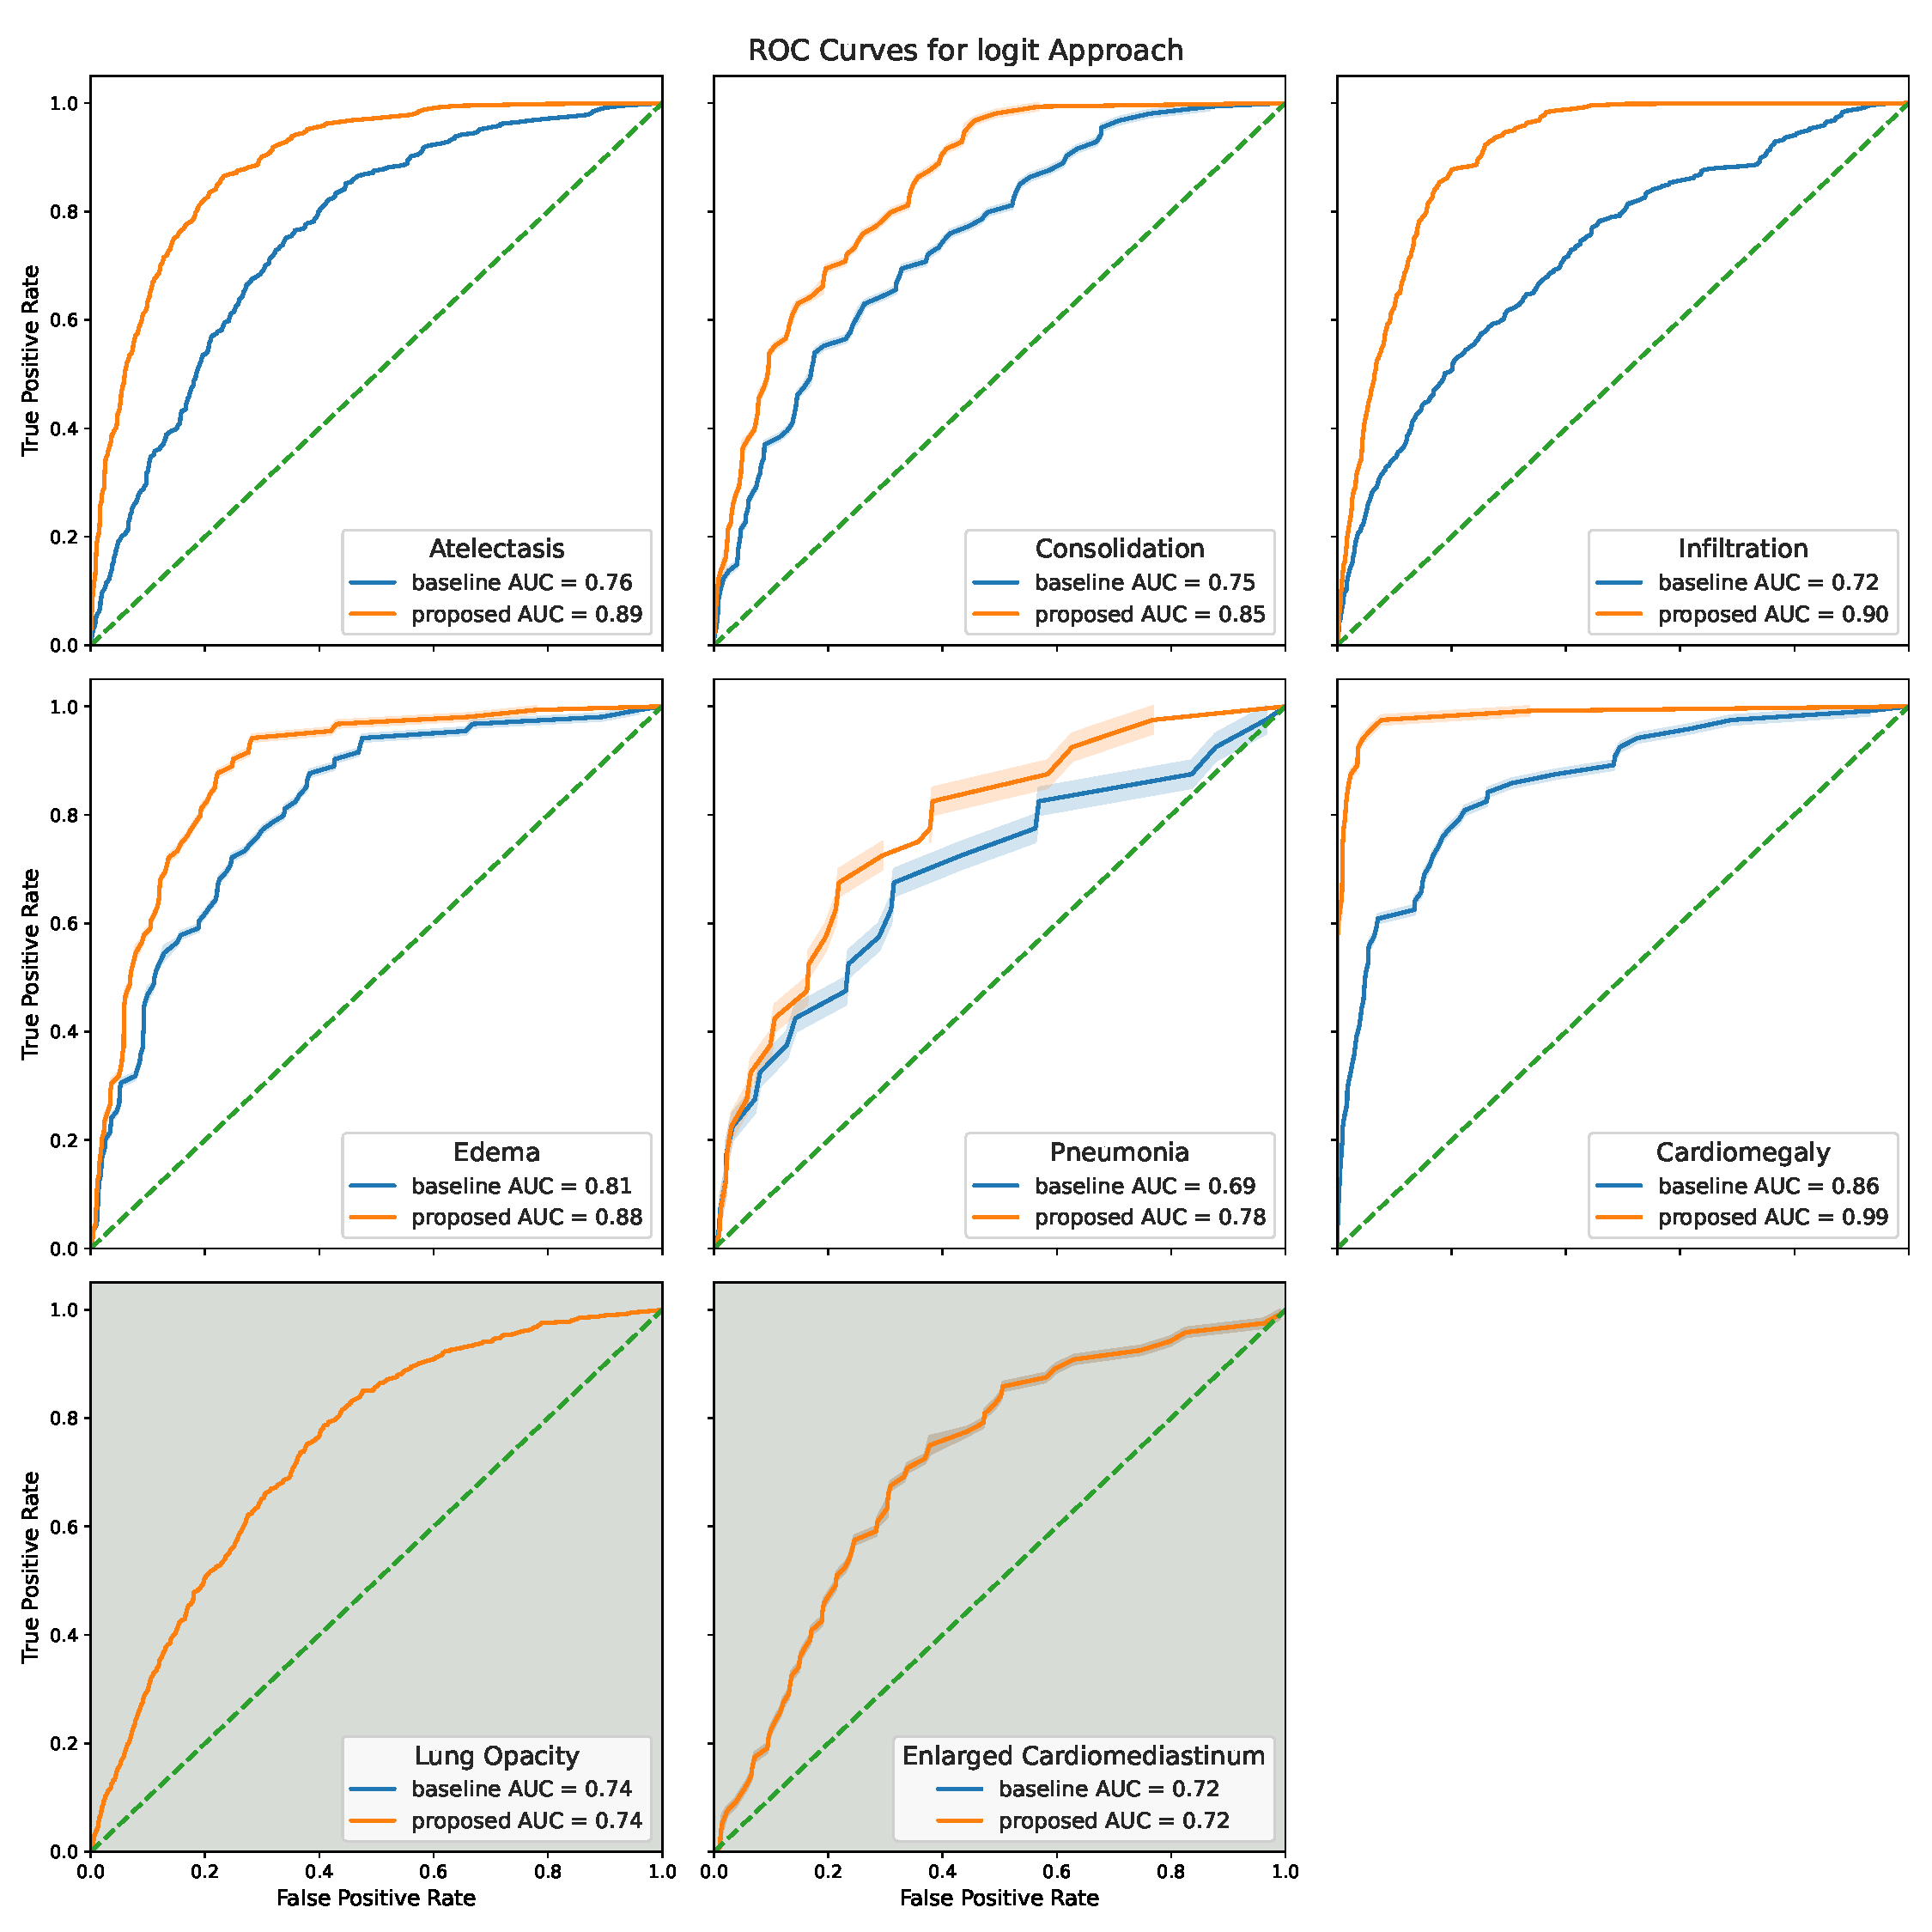
\includegraphics[width=\textwidth]{\figurepath{roc_curve/default_NIH_logit/roc_curve_NIH_logit_default.pdf}}%
    \caption{Comparative analysis of the ROC curves for eight thoracic pathologies using the baseline and the logit based proposed technique. Each subplot illustrates the overlaid ROC curves for both techniques pertaining to a specific pathology. The subplots highlighted with a darker background, represent parent class diseases.}%
    \label{Taxonomy.Fig.2.roc_curve_NIH_logit_default}
\end{figure}

Figure~\ref{Taxonomy.Fig.2.roc_curve_NIH_logit_default} illustrates a comparison between the performance of the baseline technique and the proposed logit based method (Approach 1 discussed in the Method section) in detecting eight thoracic pathologies. These eight pathologies includes the pathologies with child classes and their respective child classes as was shown in Figure~\ref{Taxonomy.Fig.1.taxonomy_structure}. The individual subplots exhibit overlaid receiver operating characteristic (ROC) curves, each of which corresponds to a specific pathology. The present analysis employed a model that was derived through the application of the test dataset from the NIH dataset to a pretrained model. The latter had undergone training on various publicly available thoracic datasets, with the aim of enabling the identification of 18 different pathologies pertaining to the thorax. The last two subplots showcased with a darker background showcases the roc curves for parent classes diseases. As these parent class diseases were not influenced by the proposed technique, their ROC curves and corresponding Area Under the Curve (AUC) values remain consistent with the baseline technique. The ROC curve and its corresponding AUC for the six child classes demonstrate a significant improvement for the proposed technique in comparison to the baseline technique.


\begin{figure}[htbp]
    \centering
    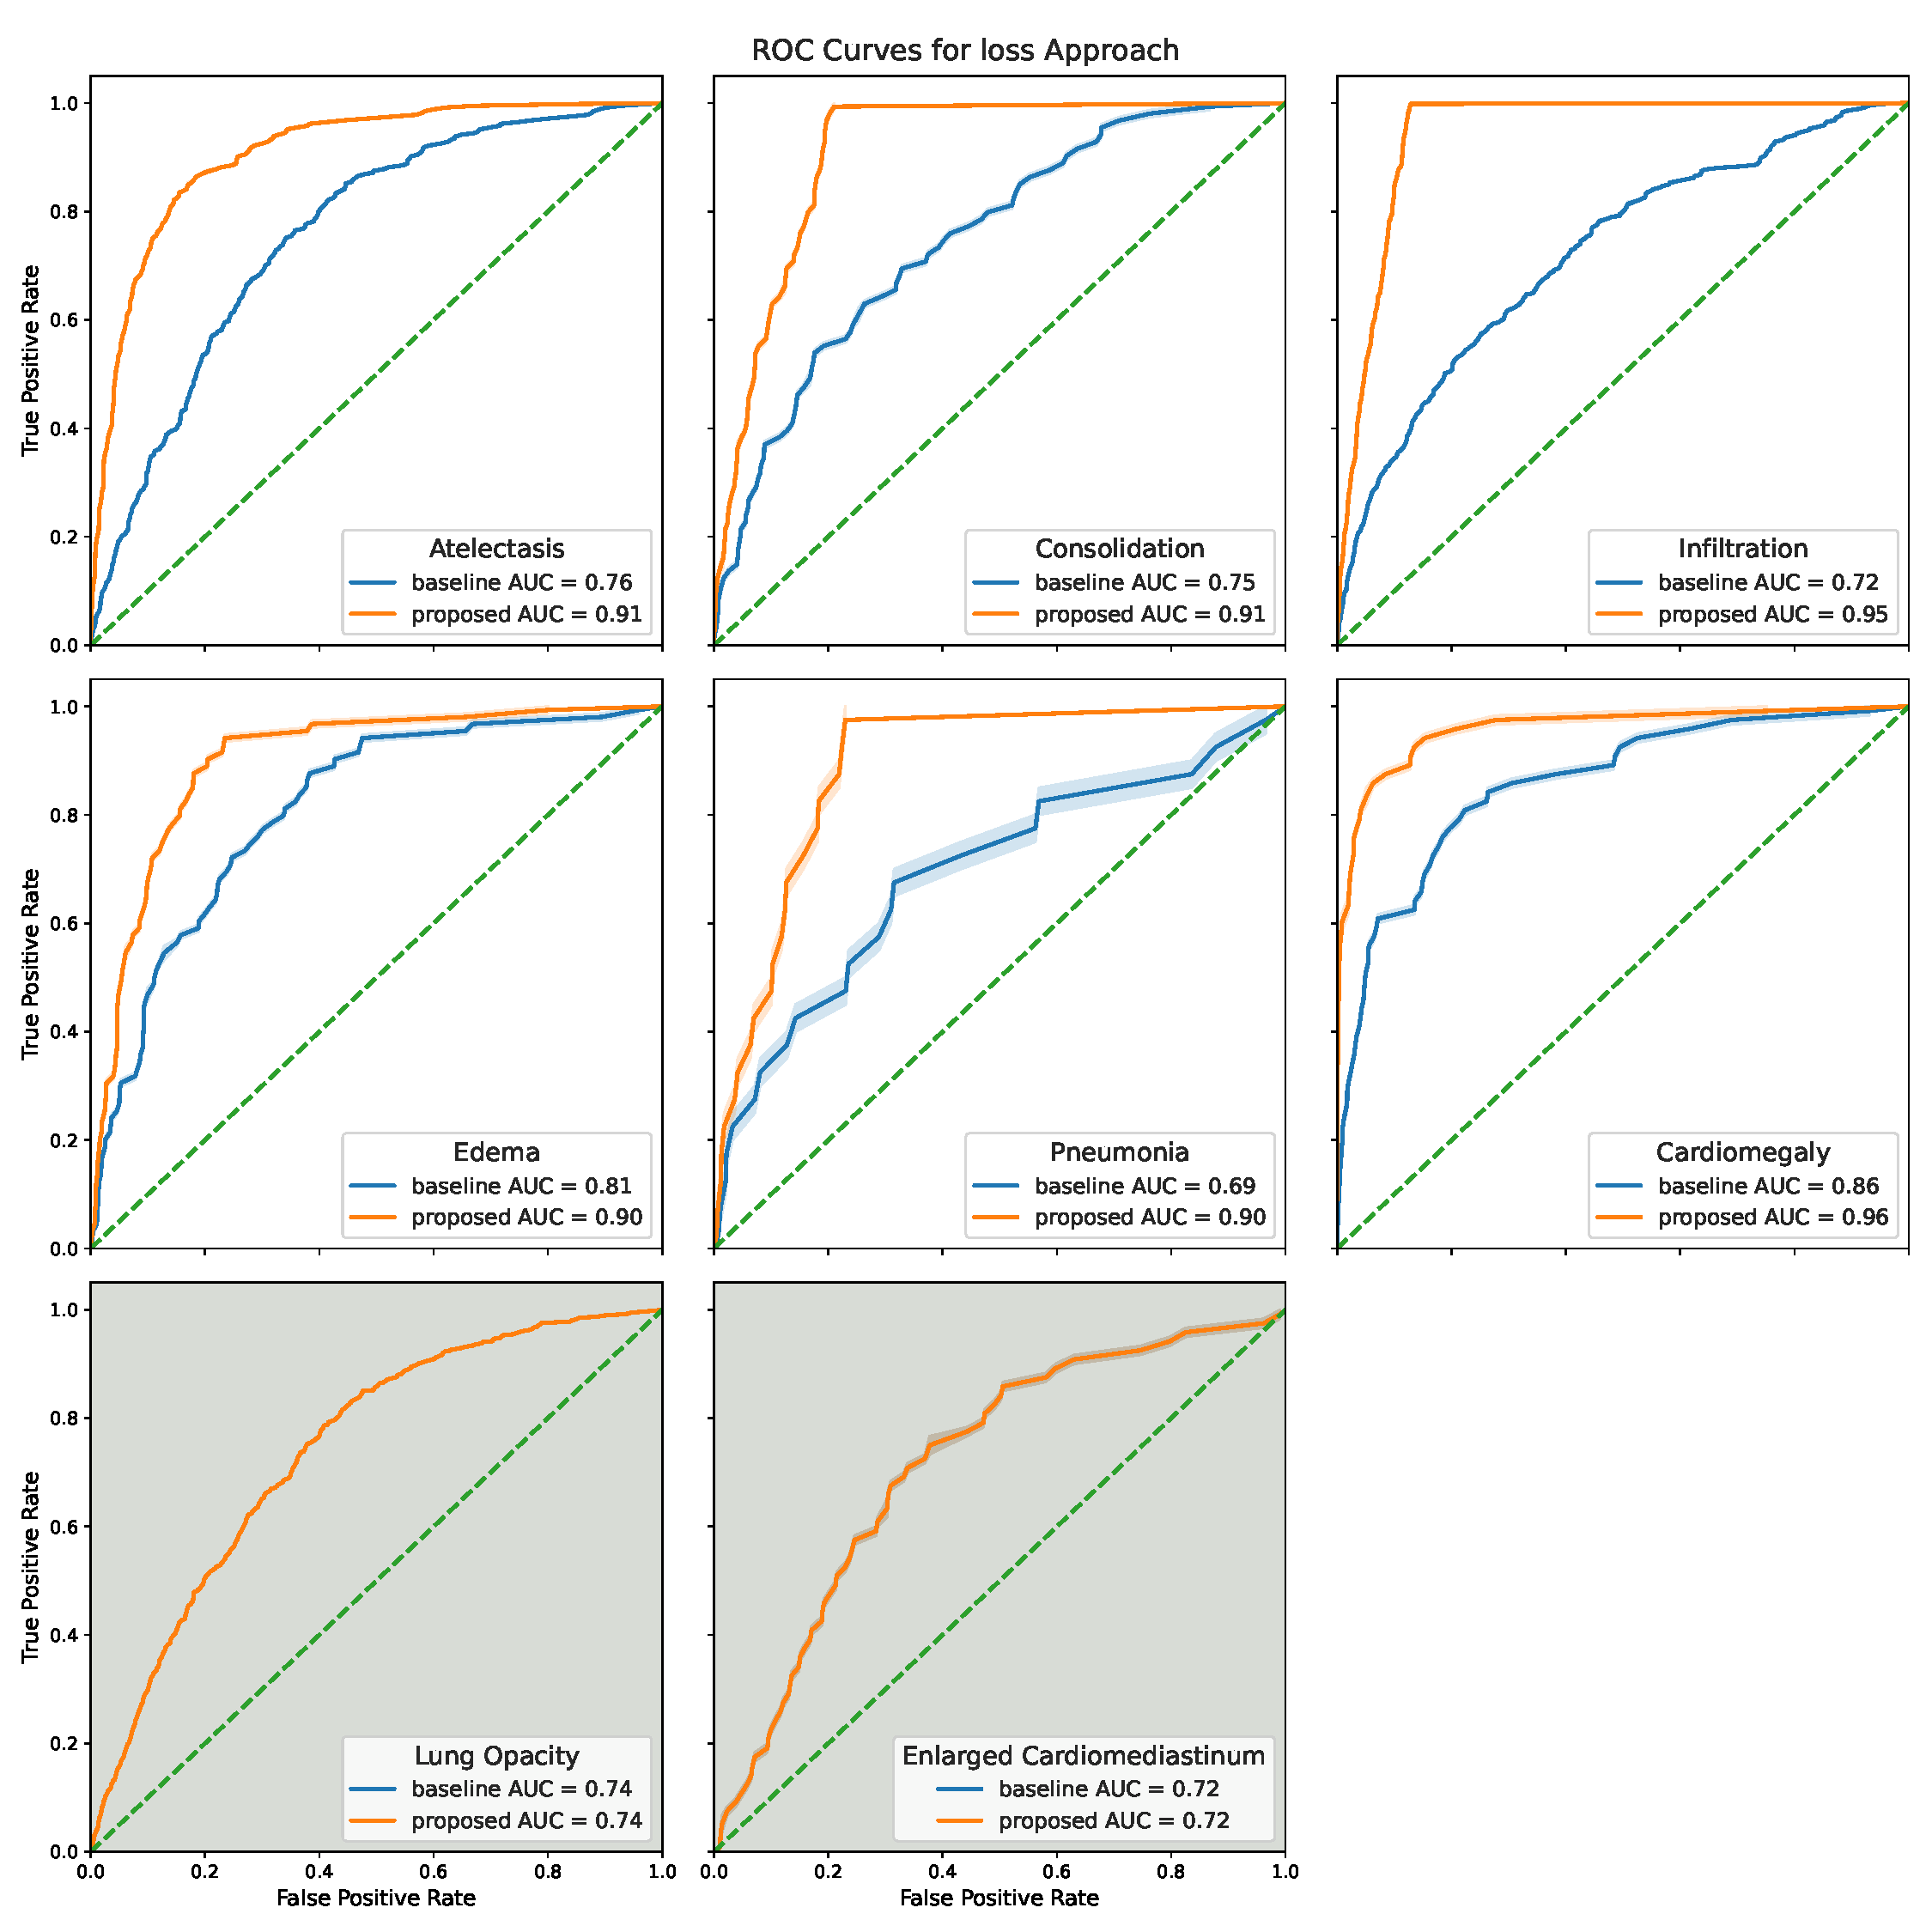
\includegraphics[width=\textwidth]{\figurepath{roc_curve/default_NIH_loss/roc_curve_NIH_loss_default.pdf}}
    \caption{Comparative analysis of the ROC curves for eight thoracic pathologies using the baseline and the loss based proposed technique. Each subplot illustrates the overlaid ROC curves for both techniques pertaining to a specific pathology. The subplots highlighted with a darker background, represent parent class diseases.}%
    \label{Taxonomy.Fig.3.roc_curve_NIH_loss_default}%
\end{figure}


Figure~\ref{Taxonomy.Fig.3.roc_curve_NIH_loss_default} illustrates a comparison between the performance of the baseline technique and the proposed loss based method (Approach 2 discussed in the Method section) in detecting eight thoracic pathologies. These eight pathologies includes the pathologies with child classes and their respective child classes as was shown in Figure~\ref{Taxonomy.Fig.1.taxonomy_structure}. The individual subplots exhibit overlaid ROC curves, each of which corresponds to a specific pathology. The present analysis employed a model that was derived through the application of the test dataset from the NIH dataset to a pretrained model. The latter had undergone training on various publicly available thoracic datasets, with the aim of enabling the identification of 18 different pathologies pertaining to the thorax. The last two subplots showcased with a darker background showcases the roc curves for parent classes diseases. As these parent class diseases were not influenced by the proposed technique, their ROC curves and corresponding AUC values remain consistent with the baseline technique. The ROC curve and its corresponding AUC for the six child classes demonstrate a significant improvement for the proposed technique in comparison to the baseline technique.

\section{Discussion and Conclusion}

\section*{Appendices}
\section*{Acknowledgements}



\bibliographystyle{apalike}
%\bibliographystyle{subfiles/bst/elsarticle-num}
\bibliography{subfiles/Better_BibTeX_Zotero}

\end{document}

% \endinput

